\scanpage{48}\mspage{47}
\uline{Definition} Let $F,\deleted{F'}G$ be two figures. We say that $\deleted{F'}G$ is a \uline{refinement} of $F$, if there exists a \deleted{\unsure{refined|raffin}} subdivision $F'$ of $F$, such that $G\subset F'$ \inserted{subfigure}.
% slanted
\margin{We write $F\ll G$}
\figure{
\begin{tikzpicture}[x=1cm,y=1cm,scale=.8]
\fill (0,0) .. controls (.1,.2) and (.16,.2) .. (.19,.55) -- (.3,.65) -- (.5,.6) .. controls (.48,.3) and (.7,.25) .. (.45,-.15) -- (.34,-.2) -- (.37,.38) -- (.12,.44) -- cycle;
\fill (1.9,.15) -- (1.85,.3) -- (2.1,.35) -- (2.35,.35) -- (2.35,.5) -- (2.55,.3) -- (2.65,.63) -- (3.35,.65) -- (3.35,.55) -- (3.5,.53) -- (3.35,.45) -- (3.45,.35) -- (3.25,.18) -- (2.7,.1) -- cycle;
\foreach \x/\y in {.6/.55,.7/.4,.4/-.28,2.1/.05,2.3/.7,2.5/-.02,3.4/.02,3.3/-.08}{\fill (\x,\y) circle(.025);}
\end{tikzpicture}}

We want this to be an order relation, and for this we are going to posit

\uline{C 4} Let $F$ be a figure, $G$ a subfigure \inserted{(i.e. $G$ a figure and $G\unsure{\subset|\in}F$)}, $G'$ a subdivision of $G$. Then \deleted{there exists a subdivision $F'$ of $F$,} \inserted{$G'\cup(F\setminus G)$ is a} subdivision \inserted{of $F$}, and the union is disjoint (i.e. \deleted{outside $G$} \margin{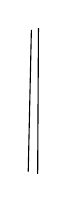
\begin{tikzpicture}[x=1cm,y=1cm]\draw (0,0)--(.04,1.8);\draw (.12,-.03)--(.13,1.82);\end{tikzpicture}}
\[
 \boxed{G'\cap F\subset G}
\]
\deleted{hence} $G'\cap F=G'\cap G$).
% slanted
\margin{This is \unsure{contradicted|obviously} \unsure{for example} the closed strata and augmented strata\ldots\ \uline{cf further} below.}
% slanted
\margin{i.e \unsure{every} multistratum of a subdivision of $G$ which is \uline{compatible} with $F$ \uline{is in $G$}. OK}
\margin{OK $\longrightarrow$}
\margin{Correct : $\exists$ subdivision which induces $G'$ $+$ the relation $G'\cap\unsure{F^{\to}\subset|F'\subset|F\subset}G$}

\uline{Corollary 1} \uline{Every} \deleted{refinement} \inserted{\uline{subdivision}} \uline{of a subfigure of $F$ is induced by a ``subdivision of $F$}.
\margin{\begin{tikzpicture}\draw (.18,0) .. controls (-.15,.25) and (-.12,.85) .. (.1,1.2);\end{tikzpicture}}

\uline{Corollary 2} The refinement relation between figures
\[
 F\ll G
\]
is an order relation.
% slanted
\margin{OK.}

\deleted{\uline{\unsure{C 5}} \inserted{\uline{Proposition}} Let $X,\deleted{\unsure{Y}}\in M$, \inserted{$\deleted{F}G\in\mathcal F$.} For $X\in\deleted{\unsure{F_Y}}G$ \deleted{i.e. $F_X\subset F_Y$} it is necessary and sufficient that $X$ and $\deleted{\unsure{Y}}G$ compatible (i.e. $F\equiv F_X\cup\deleted{\unsure{F_Y}}G$ a figure) and $X$ \deleted{refines} $\inserted{\ll}\deleted{\unsure{F_Y}}G$ i.e $F_X$ refines $\deleted{\unsure{F_Y}}G$.}
% slanted
\margin{This is the \deleted{Condition} \inserted{definition} of $\leq$ via $\ll$ and $R$}

\deleted{\deleted{\unsure{We}} Suppose indeed that $X$ and $F$ compatible \deleted{one \unsure{needs} $X\unsure{\text{and}|,|\in}Y\in F$}, $F$ a figure, and that $F_X$ refines the subfigure $F_Y\deleted{\unsure{=}} \deleted{\unsure{G.}}$. Thus $\exists$ subdivision $G'$ of}
